% % \part{优化模型}
% % \chapter{二阶椎规划SOCP}

% \documentclass[UTF8]{ctexbook}

% \ctexset{
%     part/number = \chinese{part}
% }
% \usepackage{amsmath}% ams 数学公式
% \usepackage{mathtools}% ams 数学公式
% \usepackage{amsfonts}% ams 数学字体
% \usepackage{amssymb,latexsym}% ams 数学符号与LaTeX数学符号
% \usepackage{mathrsfs}% 花式符号
% \usepackage{ntheorem}%定理、定义、证明
%   \theoremstyle{nonumberplain}
%   \theoremheaderfont{\bfseries}
%   \theorembodyfont{\normalfont}
%   \theoremsymbol{$\square$}
%   \newtheorem{Proof}{\hskip 2em 证明}
%   \newtheorem{theorem}{\hspace{2em}定理}[chapter]
%   \newtheorem{definition}{\hspace{2em}定义}[chapter] % 如果没有章, 只有节, 把上面的[chapter]改成[section]
%   \newtheorem{axiom}[definition]{\hspace{2em}公理}
%   \newtheorem{lemma}[definition]{\hspace{2em}引理}
%   \newtheorem{proposition}[definition]{\hspace{2em}命题}
%   \newtheorem{corollary}[definition]{\hspace{2em}推论}
%   \newtheorem{remark}{\hspace{2em}注}[chapter] %类似地定义其他“题头”. 这里“注”的编号与定义、定理等是分开的

% \usepackage{enumerate}%itemiz环境。\begin{enumerate}[step 1]
% \usepackage{cite}%参考文献
%     \bibliographystyle{plain}
% \usepackage{extarrows}% 带参数的箭头
% \usepackage{hyperref}% 超链接
% %\usepackage[CJKbookmarks, colorlinks, bookmarksnumbered=true,pdfstartview=FitH,linkcolor=black,citecolor=black]{hyperref}%超链接的格式设置
% \hypersetup{
%     colorlinks=false,% 去掉超链接颜色
%     pdfborder=0 0 0% 取消超链接的边框
% }
% \usepackage{graphicx}% 图片管理
% \usepackage{caption}
% \usepackage{subcaption}%并排的图各有标题
% \graphicspath{{images/}}% 设置图片搜索路径
% \usepackage{float,varwidth}% 浮动体
% \usepackage{booktabs}% 三线表
% \usepackage{fancyhdr}% 页眉设置
% \usepackage{xcolor}% 颜色宏包
% \usepackage{colortbl}% 彩色表格
% \usepackage{listings}% 代码高亮
% \usepackage{caption}% 对标题进行控制,如让\caption标题的字体缩小一号,同时数字标签使用粗体可以用:\usepackage[font=small,labelfont=bf]{caption}
% \usepackage{xfrac,upgreek}%分别是行间公式如a/b的形式(将原来的命令\frac改成\sfrac)和希腊字体的宏包的
% \usepackage{mathtools}%lgathered和rgathered环境把公式向左向右对齐
% \usepackage{tabularx}%提供自动延伸的表列,(X列格式说明符),文字过长时可以自动转行
% \usepackage{longtable}%长表格
% \usepackage{enumitem}%enumerate宏包的升级
% \usepackage{harpoon}%数学公式的矢量
% \usepackage{bookmark}%目录的书签
% \usepackage{pifont}%给数字加上圈。然后在正文输入\ding{172}~\ding{211}得到相应数字,要是要①就输入:\ding{172}②就输:\ding{173}
% \renewcommand{\headwidth}{\textwidth}%图片并排,这个要列在所有宏包的后面
% \makeatletter
% \newcommand{\rmnum}[1]{\romannumeral #1}
% \newcommand{\Rmnum}[1]{\expandafter\@slowromancap\romannumeral #1@}
% \makeatother
% \definecolor{codegreen}{rgb}{0,0.6,0}
% \definecolor{codegray}{rgb}{0.5,0.5,0.5}
% \definecolor{codepurple}{rgb}{0.58,0,0.82}
% \definecolor{backcolour}{rgb}{0.95,0.95,0.92}
% \lstset{
%     commentstyle=\color{codegreen},
%     keywordstyle=\color{magenta},
%     numberstyle=\tiny\color{codegray},
%     stringstyle=\color{codepurple},
%     basicstyle=\footnotesize,
%     breakatwhitespace=false,% 断行只在空格处
%     breaklines=true,% 自动断行
%     captionpos=b,% 标题位置
%     keepspaces=true,
%     numbers=left,
%     numbersep=5pt,
%     showspaces=false,
%     showstringspaces=false,
%     showtabs=false,% 显示
%     tabsize=2% TAB 被当作两个空格
% }
% \topmargin=0pt\oddsidemargin=0pt\evensidemargin=0pt
% \textwidth=16.5cm\textheight=23cm\raggedbottom%我这么设置是为了缩小页边距,满足有的文字无法转行
% \pagestyle{headings}%页眉为章节标题,无页脚
% \setlength{\abovecaptionskip}{4pt}
% \setlength{\belowcaptionskip}{-8pt}%图片表格的前后距离设置
% \CTEXsetup[format={\zihao{-3}\raggedright\bfseries}]{section}%设置节的格式

% \begin{document}
% \part{优化模型}
\chapter{二阶椎规划}
\section{问题的引入与分析}
    \par
    为了说明二阶椎规划的重要性,我们先将如下几个优化问题转化为二阶椎规划SOCP问题:
    \begin{enumerate}
    \item 凸二次规划的转化;
    \item 凸二次约束线性规划的转化;
    \item 凸二次约束二次规划的转化;
    \item 支持向量机的二阶锥形式;
    \end{enumerate}
    \subsection{凸二次规划的转化}
        \par
        考虑如下的严格凸二次规划问题
        \begin{align*}
          & \mathop{\min}\  f(x) = x^\mathrm{T} Qx+a^\mathrm{T} x+\beta\\
          & s.t.\left\{
            \begin{aligned}
             &Ax=b\\
             &x \geqslant 0
            \end{aligned}
             \right.
        \end{align*}
        其中:$Q$是一个对称正定矩阵,即$Q=Q^\mathrm{T}>0$;$a \in R^n,\beta \in R,A\in R^{m\times n}$。令$\bar{u}=Q^{\frac 12}x+{\frac 12}Q^{-\frac 12}a$,则目标函数$f$可以写为
        \begin{align*}
          f(x) = \|\bar{u}\|^2+\beta-\frac 14a^\mathrm{T} Q^{-1}a
        \end{align*}
        于是原问题变为
        \begin{align*}
          & \mathop{\min} \  u_0\\
          & s.t.\left\{
            \begin{aligned}
             &Ax=b\\
             &Q^{\frac 12}x-\bar{u}=-\frac 12 Q^{-\frac 12}a\\
             &(u_0;\bar{u}) \succeq 0\\
             &x \succeq 0
            \end{aligned}
             \right.
        \end{align*}
        其中:$\succeq$是定义在$\mathcal{K}$上的偏序。$\forall x,y \in \mathcal{K}$,如果$x - y \in \mathcal{K}$,记为$x \succeq \mathcal{K}_y$或$x \succeq y,x \in R^n$。
    \subsection{凸二次约束线性规划的转化}
        \par
        考虑凸二次约束线性目标规划问题
        \begin{align*}
          & \mathop{\min}\limits_x \  c^\mathrm{T} x\\
          & s.t.\left\{
            \begin{aligned}
             &x^\mathrm{T} Q_i x+a_i^\mathrm{T} x+{\beta}_i \leqslant 0\\
             &i \in I=\{1,2,\ldots,r\}
            \end{aligned}
             \right.
        \end{align*}
        其中:对$Q_i$作Cholesky分解,设$Q_i=B_iB_i^\mathrm{T} (i=0,1,\ldots,m)$,
        $B_i \in R^{k_i\times n}$,$rank(B_i)=k_i,i \in I$。
        \par
        记$q(x)=x^\mathrm{T} B^\mathrm{T} Bx+a^\mathrm{T} x+\beta \leqslant 0$,则
        \begin{align*}
          (Bx)^\mathrm{T} Bx \leqslant 1\cdot (-a^\mathrm{T} x-\beta)
        \end{align*}
        即$\|Bx\|^2 \leqslant (\frac{1-a^\mathrm{T}x -\beta}{2})^2-(\frac{1+a^\mathrm{T}x +\beta}{2})^2$。
        令
        \begin{align*}
          &u_0= \left( \frac{1-a^\mathrm{T} x-\beta}{2} \right) \\
          &\bar{u}=\begin{pmatrix} Bx \\\frac{1+a^\mathrm{T} +\beta}{2}\end{pmatrix}
        \end{align*}
        于是$q(x)=\|\bar{u}\|^2-{\mu}_0^2 \leqslant 0$。
    \subsection{凸二次约束二次规划问题QCQP}
        \par
        考虑凸二次约束二次规划问题QCQP
        \begin{align*}
          & \mathop{\min} \  x^\mathrm{T} Q_0x+a_0^\mathrm{T} x+{\beta}_0\\
          & s.t.\left\{
            \begin{aligned}
             &x^\mathrm{T} Q_ix+a_i^\mathrm{T} x+{\beta}_i \leqslant 0\\
             &i =1,2,\ldots,m
            \end{aligned}
             \right.
        \end{align*}
        其中:$a_i \in R^n$,${\beta}_i \in R$,$Q_i$为对称半正定,即$Q_i \succeq 0(i=1,2,\ldots,m)$,$x \in R^n$。
        \par
        对$Q_i$作Cholesky分解,设$Q_i=B_iB_i^\mathrm{T} (i=0,1,\ldots,m)$,则原问题变为如下二阶锥规划
        \begin{align*}
          & \mathop{\min}\ t\\
          & s.t.
          \left\{
          \begin{aligned}
          &(u_{i0};{\bar{u}}_i)\succeq 0\quad i=1,2,\ldots,m\\
          &u_{00}=\frac{1+a_0^\mathrm{T} x-{\beta}_0+t}{2}\\
          &\bar{u}=\begin{pmatrix} B_0^\mathrm{T} x \\\frac{a_0^\mathrm{T} x+{\beta}_0-t+1}{2}\end{pmatrix}\\
         & u_{i0}=\frac{1-a_i^\mathrm{T} x-{\beta}_i}{2}\\
          &{\bar{u}}_i=\begin{pmatrix} B_i^\mathrm{T} x \\\frac{a_i^\mathrm{T} x+{\beta}_i+1}{2}\end{pmatrix}
          \end{aligned}
          \right.
        \end{align*}
    \subsection{支持向量机的锥形式}
        \par
        SVM针对大规模不是十分有效,Debrath、Muramatsu和Takahashi于2005年给出了一个针对大规模问题的基于二阶锥规划的支持向量机学习方法。
        考虑二分类支持向量机的一般形式
        \begin{align*}
          & \mathop{\min}\  \frac 12 w^\mathrm{T} w+C\mathop{\sum}\limits_{i=1}^l{\xi}_i\\
          & s.t.\left\{
            \begin{aligned}
          & y_i(w^\mathrm{T} \phi(x_i)+b)\geqslant 1-{\xi}_i\\
          & {\xi}_i \geqslant 0\\
          & i=1,2,\cdots
            \end{aligned}
             \right.
        \end{align*}
        其中:$C$为罚权重,$\phi(x_i)$是一个将$x_i$映射到高维的映射,$y_i=\{-1,1\}$,$w$为优化参数,$\{x_i,y_i\}_{i=1}^l$为样本数据且已知。
        \par
        上述模型的对偶问题为
        \begin{align*}
          & \mathop{\min} \ \frac 12 {\alpha}^\mathrm{T} Q{\alpha}-e^\mathrm{T} {\alpha}\\
          & s.t.\left\{
            \begin{aligned}
          & y^\mathrm{T} {\alpha}=0\\
          & 0 \leqslant {\alpha}_i \leqslant C
            \end{aligned}
             \right.
        \end{align*}
        其中:$\alpha$为拉格朗日乘子,$e$为单位向量,$Q \geqslant 0$,$Q_{ij}=y_iy_jK(x_ix_j)$。$K(x_ix_j)=\big<\phi (x_i),\phi(x_j)\big>$是内积核。将模型重新写为
        \begin{align*}
          & \mathop{\min} \ \frac 12 {\alpha}^\mathrm{T} Q{\alpha}-e^\mathrm{T} {\alpha}\\
          & s.t.\left\{
            \begin{aligned}
          & y^\mathrm{T} {\alpha}=0\\
          & {\alpha}+\beta = Ce\\
          & {\alpha},\beta \geqslant 0\\
          & {\alpha},\beta \in R^l
            \end{aligned}
             \right.
        \end{align*}
        其中:$\beta$为松弛变量,$Q \geqslant 0$,设$Q$的秩为$r$,其Cholesky分解为$Q=BB^\mathrm{T} $,其中$B\in R^{l\times r}$,则
        \begin{align*}
          {\alpha}^\mathrm{T} Q{\alpha}={\alpha}^\mathrm{T} BB^\mathrm{T} {\alpha}=\|B^\mathrm{T} \alpha\|^2
        \end{align*}
        \par
        于是,极小化${\alpha}^\mathrm{T} Q{\alpha}$等价于在约束$\|B^\mathrm{T} \alpha\|^2$下极小化$\theta$。利用双曲约束的等价关系:
        \begin{align*}
        w^\mathrm{T}w \leqslant xy , w\in R^n ,x\in R_+,y\in R_+ \Leftrightarrow (x+y;2w;x-y) \geqslant 0
        \end{align*}
        可以把约束$\|B^\mathrm{T} \alpha\|^2 \leqslant Q$转化为
        \begin{align*}
          \left( \frac {\theta-1}{2} \right) ^2+\|B^\mathrm{T} \alpha\|^2 \leqslant \left( \frac {\theta+1}{2} \right) ^2
        \end{align*}
        令
        \begin{align*}
          & u=B^\mathrm{T} \alpha\\
          & z_1=\frac {\theta +1}{2}\\
          & z_2=\frac {\theta -1}{2}
        \end{align*}
        则模型定为
        \begin{align*}
          & \mathop{\min}\  \frac 12 (z_1+z_2)-e^\mathrm{T} {\alpha}\\
          & s.t.\left\{
            \begin{aligned}
          & y^\mathrm{T} {\alpha}=0\\
          & {\alpha}+\beta = Ce\\
          & G^\mathrm{T} {\alpha}-u=0,u \in R^r\\
          & z_1-z_2=1\\
          & {\alpha},\beta \geqslant 0\\
          & z_1^2\geqslant z_2^2+\|w\|^2
            \end{aligned}
             \right.
        \end{align*}
        上述问题是一个二阶锥规划。
        % 整体写为
        % \begin{align*}
        %   & \mathop{\min} \ \left[-e^\mathrm{T} ,0,\frac 12,\frac 12,0\right] \begin{bmatrix} \alpha \\\beta\\z_1\\z_2\\u\end{bmatrix}\\
        %   & s.t.\left\{
        %     \begin{aligned}
        %   &\begin{bmatrix} y^\mathrm{T} & 0 & 0 & 0 & 0 \\I&I&0&0&0\\G^\mathrm{T} & 0 & 0 & 0 & -I \\0& 0 & 1 & -1 & 0 \end{bmatrix}\begin{bmatrix} \alpha \\\beta\\z_1\\z_2\\u\end{bmatrix}=\begin{bmatrix} 0 \\Ce\\0\\1\end{bmatrix}\\
        %   & {\alpha},\beta \geqslant 0\\
        %   & z_1^2\geqslant z_2^2+\|u\|^2
        %     \end{aligned}
        %      \right.
        % \end{align*}
\section{模型规范化及其基本理论}
    \subsection{二阶椎和二阶椎规划的定义}
        \begin{definition}[二阶锥]
        二阶锥又称为Lorentz锥,$n$维二阶锥$\mathcal{K}^n$的定义为
        \begin{align*}
          \mathcal{K}^n=\{(x_1,x_2) \in R\times R^{n-1}|x_1 \geqslant \|x_2\|\}
        \end{align*}
        其中:$\|\cdot\|$为$L_2$范数,如果是其它范数,亦可定义其它锥。
        \end{definition}
        \par
        定义二阶锥内部为
        \begin{align*}
          {int}\mathcal{K}^n=\{(x_1,x_2) \in R\times R^{n-1}|x_1 > \|x_2\|\}
        \end{align*}
        不难看出在$R,R^2,R^3$中二阶锥的形状,如图(\ref{fig:三维二阶锥示意图})所示
                \begin{figure}[H]
                \centering
                \begin{subfigure}[b]{0.3\textwidth}
                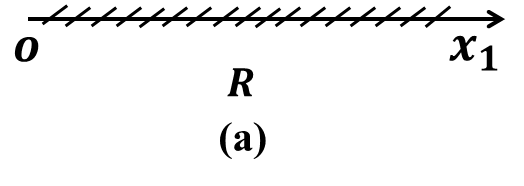
\includegraphics[width=\textwidth]{images/Three_dimensional_2order_cone1.jpg}
                \end{subfigure}
                \begin{subfigure}[b]{0.3\textwidth}
                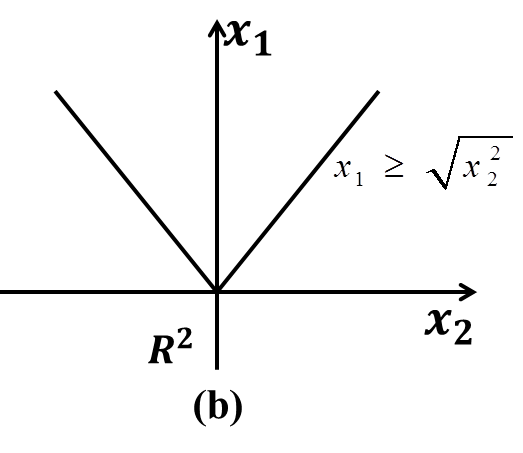
\includegraphics[width=\textwidth]{images/Three_dimensional_2order_cone2.jpg}
                \end{subfigure}
                \begin{subfigure}[b]{0.3\textwidth}
                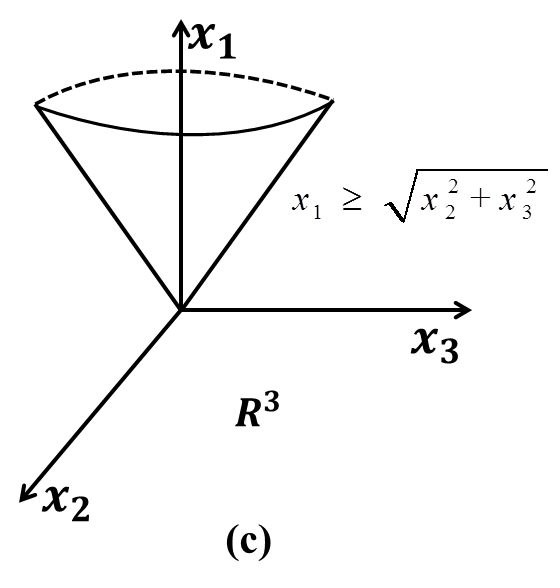
\includegraphics[width=\textwidth]{images/Three_dimensional_2order_cone3.jpg}
                \end{subfigure}
            \caption{三维二阶锥示意图}
            \label{fig:三维二阶锥示意图}
            \end{figure}
        \par
        上面给出了二阶锥$K$的定义,二阶锥规划就是在二阶锥内求变量$x$使目标最优,即最优化模型的约束条件为二阶锥条件。
        \par
        二阶锥规划的标准形式为
        \begin{align*}
          & \mathop{\min} \ \mathop{\sum}\limits_{i=1}^rC_i^\mathrm{T} x_i\\
          & s.t.\left\{
            \begin{aligned}
          & \mathop{\sum}\limits_{i=1}^rA_ix_i=b_i\\
          & x_i \in \mathcal{K}^{n_i}\\
          & i \in I
            \end{aligned}
             \right.
        \end{align*}
        其中:$I=\{1,2,\ldots,r\}$,$b \in R^m$,$C_i \in \mathcal{K}^{n_i}$,$A_i \in R^{m\times n_i}$,$\mathcal{K}^{n_i}=\{(x_{i1},{\bar{x}}_i) \in R^{n_i}|x_{i1}\geqslant \|{\bar{x}}_i^\mathrm{T} \| \}$,$x_i=(x_{i1},{\bar{x}}_i)$表示$(x_{i1} ,{\bar{x}}_i^\mathrm{T} )^\mathrm{T} $,且${\bar{x}}_i=(x_{i2},x_{i3},\ldots,x_{in_i},)$。
        % 一般形式的SOCP为
        % \begin{align*}
        % &\min_x \  C^\mathrm{T}X\\
        % &s.t.\left\{
        % \begin{aligned}
        % &AX-B = 0\\
        % &A_iX - b_i \preceq K^{n_i}
        % \end{aligned}
        % \right.
        % \end{align*}
        % 其中:$K^{n_i}$是$R^{n_i}$中的二阶锥。

    \subsection{拉格朗日对偶问题}
        \par
        为得到上述问题的对偶形式,将$x_i \in \mathcal{K}^{n_i}$转化为
        \begin{align*}
          & \mathop{\sum} \limits_{j=2}^{n_i}x_{ij}^2-{\bar{x}}_i^2\leqslant 0\text{及} x_{i1}\geqslant 0
        \end{align*}
        对$u_i\geqslant 0,i \in I$,有
        \begin{align*}
          u_i \left( \mathop{\sum} \limits_{j=2}^{n_i}x_{ij}^2-{\bar{x}}_i^2 \right) =-\left[(u_ix_{i1})x_{i1}+\left( \mathop{\sum} \limits_{j=2}^{ni}(-u_ix_{i1})x_{ij} \right) \right]
        \end{align*}
        我们设
        \begin{align*}
         s_i=(u_ix_{i1},-u_ix_{i2},\ldots,u_ix_{in_i})^\mathrm{T} \in R^{n_i}
        \end{align*}
        显然$s_i \in \mathcal{K}^{n_i}$,且
        \begin{align*}
         u_i \left( \mathop{\sum} \limits_{j=2}^{n_i}x_{ij}^2-x_{i1}^2 \right) =-s_i^\mathrm{T} x_i \quad i \in I
        \end{align*}
        于是原问题的Lagrange对偶函数为
        \begin{align*}
         \theta(s_i,y)&=\inf\left\{\mathop{\sum} \limits_{i=1}^{r}c_i^\mathrm{T} x_i-\mathop{\sum} \limits_{i=1}^{r}s_i^\mathrm{T} x_i+y^\mathrm{T} \left(b-\mathop{\sum} \limits_{i=1}^{r}A_ix_i\right)\right\}\\
         &=\inf\left\{\mathop{\sum} \limits_{i=1}^{r}(c_i-s_i-A_i^\mathrm{T} y)^\mathrm{T} x_i+b^\mathrm{T} y\right\}
        \end{align*}
        其中:$y \in R^m$。当$c_i-s_i-A_i^\mathrm{T} y=0$时,$\theta(s_i,y)=b^\mathrm{T} y$,故对偶问题可描述为
        \begin{align*}
          & \mathop{\max}\ b^\mathrm{T} y\\
          & s.t.\left\{
            \begin{aligned}
          & A_i^\mathrm{T} y+s_i=c_i \quad i\in I\\
          & s_i \in \mathcal{K}^{n_i}
            \end{aligned}
             \right.
        \end{align*}
        这里,$s_i$为松弛变量,$y \in R^{m}$为决策变量。
        \par
        令
        \begin{align*}
          & \mathcal{K}=\mathcal{K}^{n_1}\times \mathcal{K}^{n_2}\times\cdots \times \mathcal{K}^{n_r}\\
          & A=(A_1,A_2,\cdots,A_r)\in R^{m\times n}\\
          & C=(c_1,c_2,\cdots,c_r)\in R^ n \\
          & x=(x_1,x_2,\cdots,x_r)\in K\\
          & s=(s_1,s_2,\cdots,s_r)\in K\\
          & n=n-1+n_2+\cdots+n_r
        \end{align*}
        则原二阶锥规划及其对偶问题可简写为如下形式
        \begin{align*}
          & \mathop{\min}\{c^\mathrm{T} x|Ax=b,x \in \mathcal{K}\}\\
          & \mathop{\max}\{b^\mathrm{T} y|A^\mathrm{T} y+s=c,s \in \mathcal{K}\}
        \end{align*}
        注:假设$A$是行满秩的,即$rank(A)=m,m \leqslant n$。
        \par
        二阶锥规划(SOCP)介于线性规划和半正定规划之间,属于凸优化问题。目标函数是线性函数,约束是一个仿射空间和有限个二阶锥的笛卡尔积交空间。
    \subsection{二阶锥规划的研究进展}
        todo:未完成:引入最优化基础.docx的5-5.2。
    \subsection{最优化条件及对偶定理}
        \par
        作为研究二阶锥规划的代数基础,欧几里得约当(Jordan)代数显示了它独有的功效。1994年Faraut和Koranyi在《Analysis on Symmetric Cones》中指出:\textbf{Jordan代数}使线性规划、半定规划和二阶锥规划有了统一的理论基础。Alizadeh和Goldfard在《second-order-conc programming》中提出了针对二阶锥规划的Jordan代数,指出对它们的理解可使人们观察到二阶锥规划问题的所有方面:从对偶性、互补性到非退化条件,最终到内点法的设计与分析。下面给出论文中的一些结论,为了书写方便,令$\mathcal{K}=\mathcal{K}^n$。对于任意的$x=(x_1,\bar{x})\in R\times R^{n-1}$和$s=(s_1,\bar{s})\in R\times R^{n-1}$,与二阶锥$\mathcal{K}$相伴的Jordan积定义为
        \begin{align*}
          & x \circ s=(x^\mathrm{T} s,x_1\bar{s}+s_1\bar{x})
        \end{align*}
        对上述的Jordan积($R^n,\circ$),有如下性质\footnote{
        注:Jordan积'$\circ$'一般不满足结合律,即$\forall x,y,z\in R^n$。
        \begin{align*}
          (x\circ y)\circ z \neq x\circ (y\circ z)
        \end{align*}
        但在内积定义下,结合律成立
        \begin{align*}
          \big< {x, y\circ z} \big> = \big<{x\circ y,z} \big>
        \end{align*}
        }:\par
        (1)\ 对$\forall \alpha,\beta \in R$,有分配律
        \begin{align*}
          & x \circ (\alpha y+\beta z)=\alpha x\circ y+\beta x\circ z\\
          & (\alpha y+\beta z)\circ x=\alpha y\circ x+\beta z \circ x
        \end{align*}
        \par
        (2)\ $x\circ s=s\circ x$;\par
        (3) 设向量$e$为唯一的单位元,$e=(1,0,\ldots,0)^\mathrm{T} \in R^n$
        \begin{align*}
          x\circ e=e\circ x=x
        \end{align*}
        \par
        (4) 令$x^2=x \circ x$,则$\forall s \in R^n$,有$x\circ (x^2\circ s)=x^2\circ (x\circ s)$。
        \par
        \begin{definition}[向量特征值]
        $\forall x=(x_1,\bar{x})\in R\times R^{n-1}$,有
        \begin{align*}
          x^2-2x_1x+(x_1^2+\|\bar{x}\|^2)e=0
        \end{align*}
        我们称多项式
        \begin{align*}
          P(\lambda,x)={\lambda}^2-2x_1\lambda+(x_1^2-\|\bar{x}\|^2)=0
        \end{align*}
        为$x$的特征多项式,并且称特征多项式的两个根${\lambda}_{1}(x)=x_1-\|\bar{x}\|$和${\lambda}_{2}(x)=x_1+\|\bar{x}\|$为$x$的特征值。
        \end{definition}
        \par
        对$\forall x \in R^n$,易证明下面的等式成立
        \begin{align*}
          x=\frac 12 (x_1-\|\bar{x}\|)\begin{pmatrix} 1 \\-\frac{\bar{x}}{\|\bar{x}\|}\end{pmatrix}+\frac 12 (x_1+\|\bar{x}\|)\begin{pmatrix} 1 \\\frac{\bar{x}}{\|\bar{x}\|}\end{pmatrix}
        \end{align*}
        \begin{definition}[特征值分解]$\forall x = (x_1,\bar{x})\in R\times R^{n-1}$,其特征值分解为
        \begin{align*}
          x={\lambda}_1(x)u^{(1)}+{\lambda}_2(x)u^{(2)}
        \end{align*}
        其中:特征值${\lambda}_1(x)=x_1-\|\bar{x}\|,{\lambda}_2(x)=x_1+\|\bar{x}\|$。
        特征向量($i =1,2$)
        \begin{align*}
          & u^{(i)}=\left\{
            \begin{aligned}
          &\frac 12 \left( 1-(-1)^i \frac{\bar{x}}{\|\bar{x}\|} \right) \quad \bar{x}\neq 0\\
          &\frac 12 \left( 1-(-1)^i w \right) \quad \bar{x} = 0
            \end{aligned}
             \right.
        \end{align*}
        这里,$w \in R^{n-1}$是满足$\|w\|=1$的任意向量。
        \end{definition}
        \par
        易知
        \begin{align*}
          & x \in \mathcal{K}\Leftrightarrow {\lambda}_2(x) \geqslant {\lambda}_1(x) \geqslant 0\\
          & x \in int{}\mathcal{K}\Leftrightarrow {\lambda}_2(x) \geqslant {\lambda}_1(x) > 0
        \end{align*}
        注意到,$u^{(1)},u^{(2)}$属于$\mathcal{K}$,但不属于$int \mathcal{K}$。此外
        \begin{align*}
          & u^{(1)}\circ u^{(2)}=0,u^{(1)}+u^{(2)}=e,\|u^{(1)}\|=\|u^{(2)}\|=\frac {1}{\sqrt{2}}\\
          & u^{(1)}\circ u^{(1)}=u^{(1)},u^{(2)}\circ u^{(2)}=u^{(2)}
        \end{align*}
        \par
        利用向量的特征值分解,可以定义\par
        \ding{172}绝对值:$|x|=|{\lambda}_1(x)| u^{(1)}+|{\lambda}_2(x)| u^{(2)},\forall x \in \mathcal{K}$;\par
        \ding{173}平方:$x^2={\lambda}_1(x)^2 u^{(1)}+{\lambda}_2(x)^2 u^{(2)}$;\par
        \ding{174}平方根:$\sqrt{x}=\sqrt{{\lambda}_1(x)} u^{(1)}+\sqrt{{\lambda}_2(x)} u^{(2)},$;\par
        \ding{175}逆:$x^{-1}={\lambda}_1(x)^{-1} u^{(1)}+{\lambda}_2(x)^{-1} u^{(2)}$。
        \par
        容易证明下列关系式成立
        \begin{align*}
           |x|=\sqrt{x^2},\quad x^2=x \circ x,\quad (\sqrt{x})^2=x
        \end{align*}
        并且,如果$x^{-1}$存在,则称$x$可逆,且满足$x \circ x^{-1}=e$。
        \par
        对任意的$x=(x,\bar{x})\in R\times R^{n-1}$,其行列式和迹分别定义为
        \begin{align*}
           \det(x)={\lambda}_1(x){\lambda}_2(x)=x_1^2-\|\bar{x}\|^2\\
           \mathrm{Tr}(x)={\lambda}_1(x)+{\lambda}_2(x)=2x_1
        \end{align*}
        \par
        对任意的$x=(x,\bar{x})\in R\times R^{n-1}$,定义对称矩阵
        \begin{align*}
           L_x=\begin{pmatrix} x & \bar{x}^\mathrm{T} \\\bar{x} & x_1I\end{pmatrix}\in R^{n\times n}
        \end{align*}
        其中:$I$为${n-1}\times {n-1}$的单位矩阵。
        有
        \begin{align*}
          & x\circ s=s\circ x=L_xs=L_sx=L_xL_se
        \end{align*}
        这里,当且仅当$x \in \mathcal{K}(x \in int {} \mathcal{K})$时,$L_x$是半正定矩阵(正定矩阵)。此外,如果$x \in int{}\mathcal{K}$,那么矩阵$L_x$可逆:
        \begin{align*}
           L_x^{-1}=\frac {1}{\det(x)}\begin{pmatrix} x_1 & -\bar{x}^\mathrm{T} \\-\bar{x} & \frac{\det(x)}{x_1}I+\frac{\bar{x}{\bar{x}}^\mathrm{T} }{x_1}\end{pmatrix}
        \end{align*}
        \par
        上面分析了$\mathcal{K}$为单一二阶锥的情况,所有结论可平行推广到$\mathcal{K}=\mathcal{K}^{n_1}\times \mathcal{K}^{n_2}\times\cdots \mathcal{K}^{n_r}$的情形。令$x=(x_1\cdots x_r)$,$s=(s_1\cdots s_r)$,$x_i,s_i\in \mathcal{K}^{n_i}$,$i=(1,2,\cdots,r)$,则\par
        (1)\ $x\circ s=(x_1\circ s_1,\cdots,x_r\circ s_r)$;\par
        (2)\ $L_x=diag(L_{x_1},L_{x_2},\cdots,L_{x_r})$;\par
        (3)\ $\mathrm{Tr}(x)=\mathop {\sum}\limits_{i=1}^r \mathrm{Tr}(x_i)=\mathop {\sum}\limits_{i=1}^r[{\lambda}_1(x_i)+{\lambda}_2(x_i)]$;\par
        (4)\ $\det(x)=\mathop {\prod}\limits_{i=1}^r \det(x_i)=\mathop {\prod}\limits_{i=1}^r{\lambda}_1(x_i)+{\lambda}_2(x_i)$;\par
        (5)\ $x$的特征值具有$2r$个(含多重特征值,由$x_1,\cdots,x_r$的特征值构成);\par
        (6)如果$x_i \in int \mathcal{K}^{n_i}$,则$x^{-1}=(x_1^{-1},\cdots,x_r^{-1})$。
        \par
        上面介绍了一些欧几里得约当(Jordan)代数在二阶锥问题中的一些具体理论。下面,我们利用这些理论来分析二阶锥规划最优性条件及对偶理论。并在此基础上介绍一些最优化算法。
        \paragraph{弱对偶定理}设$x$和$(y,s)$分别为二阶锥规划原问题和对偶问题的可行解,则对偶间隙为
        \begin{align*}
           c^\mathrm{T} x-b^\mathrm{T} y=x^\mathrm{T} s \geqslant 0
        \end{align*}
        \paragraph{强对偶定理}如果二阶锥原问题和对偶问题均存在严格可行解,则原问题和对偶问题存在最优解$x^*$和$(y^*,s^*)$,并且$p^*=c^\mathrm{T} x^*=b^\mathrm{T} y^*=d^*$。这里:$p^*,d^*$为原始问题(P)和对偶问题(D)的最优解。
        \paragraph{半强对偶定理}如果原问题存在严格可行解,并且其目标函数值在可行域内有下界,则对偶问题可解,且$p^*=d^*$。
        \paragraph{互补条件}对$\forall x=(x_1\cdots x_r) \in \mathcal{K},s=(s_1\cdots s_r) \in \mathcal{K} $,$x_i \in \mathcal{K}^{n_i},s_i \in \mathcal{K}^{n_i},i=1,2,\cdots,r$,使$x^\mathrm{T} s=0$,当且仅当$x_i\circ s_i=0$,即
        \par
        (i) $x_i^\mathrm{T} s_i=x_{i1}s_{i1}+{\bar{x}}_i^\mathrm{T} {\bar{s}}_i=0$\par
        (ii) $x_{i1}{\bar{s}}_i+s_{i1}{\bar{x}}_i=0$
        \paragraph{KKT条件 - 最优化条件}假设原问题和对偶问题存在严格可行解,则$(x,y,s)$是其最优解的充要条件是
        \begin{align*}
           & Ax=b\quad x \in \mathcal{K}\\
           & A^\mathrm{T} y+s=c \quad s \in \mathcal{K}\\
           & x \circ s=0
        \end{align*}
\section{最优化算法}
    \par
    内点算法是求解二阶锥规划最有效的方法之一。内点法要求初始搜索点在可行域内(如何选取$x_0$?)。2004年Zhou和Toh在《Polynomiality of an inexact infeasile interior point algorithm for semidefinte Programming》中提出一种求解半定规划的非精确不可行内点算法,此方法可推广到二阶锥规划中,但其初始点的选取受到某个最优解的限制。1996年,Nemirovskii和Scheinberg在《Extension of Karmarkar's algorithm onto convex quadratically constrained quadratic problems》中证明了线性规划的原始对偶内点法可推广到二阶锥规划中。1994年Adler和Alizadeh研究了求解半定规划和二阶锥规划统一的原始—对偶方法,提出了适用于二阶锥规划的搜索方向。2000年,Monteiro和Tsudiya介绍了确定二阶锥规划AHO搜索方向的牛顿方程组,给出了沿AHO方向的二阶锥规划的预估—校正算法的多项式收敛性。
    \subsection{原始 - 对偶内点算法}
        \par
        内点法通常称为严格可行内点算法,因为算法所产生的所有迭代点都严格可行,其基本思想是:在可行域内选取中心路径的一个领域,算法始终追踪在这个邻域内。原始—对偶内点法的基本思想是:在中心路径附近取一个初始点,然后求一个搜索方向使对偶间隙能够减小。
        \par
        记原始规划和对偶规划的可行解与严格可行解为
        \begin{align*}
           & \mathscr{F}(P)=\{x|Ax=b,x \in \mathcal{K}\}\\
           & \mathscr{F}(D)=\{(y,s)|A^\mathrm{T} y+s=c,s \in \mathcal{K}\}\\
           & \mathscr{F}^0(P)=\{x|Ax=b,x \in int{}\mathcal{K}\}\\
           & \mathscr{F}^0(D)=\{(y,s)|A^\mathrm{T} y+s=c,s \in int{}\mathcal{K}\}
        \end{align*}
        假设:$\mathscr{F}^0(P)\times \mathscr{F}^0(D) \neq 0$,且$A$的行向量是线性无关的。由强对偶定理可知,P和D都存在最优解,且最优值相等。此外,解P和D等价于求解KKT条件
        \begin{align*}
           & Ax=b\quad x \in \mathcal{K}\\
           & A^\mathrm{T} y+s=c\quad s \in \mathcal{K}\\
           & x \circ s=0
        \end{align*}
        \par
        定义向量值函数$F:R\times R^m\times R\to R^{2n+m}$
        \begin{align*}
        F(x,y,s) =
        \begin{pmatrix}
        Ax-b\\
        A^\mathrm{T}y + s - c\\
        x\circ s
        \end{pmatrix}
        \end{align*}
        则有$F(x,y,s) = 0 $。把KKT条件加以扰动,有
        \begin{align*}
           & Ax=b\quad x \in \mathcal{K}\\
           & A^\mathrm{T} y+s=c\quad s \in \mathcal{K}\\
           & x \circ s=\mu e
        \end{align*}
        上述方程称为中心路径方程。
        \par
        已证明,上述方程对任意$\mu > 0$都有唯一解$(x(\mu),y(\mu),s(\mu))$,当$\mu$取遍所有正数时,这些解的轨迹称为\underline{中心路径}。
        在中心路径方程中,分别以$x+\Delta x,y+\Delta y,s+\Delta s$代替$x,y,s$,并去掉含$\Delta x,\Delta s$的非线性项,得到
        \begin{align*}
           & A\Delta x=r_p=b-Ax\\
           & A^\mathrm{T} \Delta y+\Delta s=r_d=c-A^\mathrm{T} y-s\\
           & L_x\Delta s+L_s\Delta x=\mu e-L_xs
        \end{align*}
        上式又可以写成矩阵形式
        \begin{align*}
           \begin{pmatrix} A & 0 & 0\\0 & A^\mathrm{T}  & I\\L_s & 0 & L_x\end{pmatrix}\begin{pmatrix} \Delta x \\ \Delta y \\ \Delta s \end{pmatrix}=\begin{pmatrix} r_p \\ r_d \\ r_c \end{pmatrix}
        \end{align*}
        解上述方程,即可得到搜索方向$(\Delta x , \Delta y , \Delta s)$
        \begin{align*}
           & \Delta y = (AL_s^{-1}L_xA^\mathrm{T} )[r_p+AL_s^{-1}(L_xr_d-r_c)]\\
           & \Delta s = r_d-A^\mathrm{T} \Delta y\\
           & \Delta x = -L_s^{-1}(L_x\Delta s-r_c)
        \end{align*}
        在此基础上,我们给出中心路径邻域的概念:
        \begin{align*}
           & L_x = diag(L_{x_1},\cdots,L_{x_r})\\
           & L_{x_i} = \begin{pmatrix} x_i & {\bar{x}}_i^\mathrm{T}  \\ {\bar{x}}_i & x_{i1}I \end{pmatrix}
        \end{align*}
        对$\forall x,s\in R^n$,定义
        \begin{align*}
           & {\beta}_{xi} = \sqrt{x_{i1}^2-\|{\bar{x}}_i\|^2}\\
           & T_{x_i} = \begin{pmatrix} x_{i1} & {\bar{x}}_i^\mathrm{T}  \\ {\bar{x}}_i & {\beta}_{xi}I+\frac{{\bar{x}}_i{\bar{x}}_i^\mathrm{T} }{{\beta}_{x_i}x_{i1}} \end{pmatrix}\\
           & T_x=diag(T_{x_1},\cdots,T_{x_r})\\
           & W_{xs} = (w_1,\cdots,w_r)=T_{x}s
        \end{align*}
        且
        \begin{align*}
           & W_{xs} = L_{w_x}s\\
           & R_{xs} = T_{x}L_{x}^{-1}L_sT_x\\
           & {\lambda}_i^1(W_{xs})=w_{i1}-\|{\bar{w}}_i\|\\
           & {\lambda}_i^2(W_{xs})=w_{i1}-\|{\bar{w}}_i\|
        \end{align*}
        对$\forall (x,s)\subset int{}\mathcal{K}\times int{}\mathcal{K}$,定义距离如下
        \begin{align*}
           & d_{2}(x,s) = \sqrt{2}\|W_{xs}-\mu e\|\\
           & d_{\infty}(x,s) = \mathop{\max}\limits_{\substack{i=1,2,\ldots,r\\j=1,2}}|{\lambda}_i^{-j}(W_{xs})-\mu |
        \end{align*}
        给定常数$\beta \in (0,1)$,定义中心路径的邻域为
        \begin{align*}
           & N_{2}(\beta) = \{(x,s)\in \mathscr{F}^0(P)\times \mathscr{F}^0(D)|d_2(x,s)\leqslant \beta \mu\}\quad \beta = \gamma\quad \tau=\mu\\
           & N_{\infty}(\beta) = \{(x,s)\in \mathscr{F}^0(P)\times \mathscr{F}^0(D)|d_{\infty}(x,s)\leqslant \beta \mu\}
        \end{align*}
        显然,$d_{\infty}(x,s)\leqslant d_2(x,s)$,所以$N_{2}(\beta)\subset N_{\infty}(\beta)$。下面,给出基于AHO搜索方向与路径跟踪内点法:\\
        \textbf{step1.}初始化。\par
        路径参数$\beta \in (0,\frac 15)$,$\delta \in (0,1)$,满足
        \begin{align*}
        \frac{\varphi({\beta}^2+{\delta}^2)}{(1-3\beta)^2}\leqslant \left( 1-\frac{\delta}{\sqrt{2r}} \right) \beta
        \end{align*}
        令$\sigma = 1-\frac{\delta}{\sqrt{2n}}$,$\varepsilon \in (0,1)$。初始点$(x_0,y_0,s_0)\in N(\beta)$
        \begin{align*}
        {\mu}_0=\frac{x_0^\mathrm{T} y_0}{r}
        \end{align*}
        置$k:=0$。\\
        \textbf{step2.}计算搜索方向$(\Delta x^k,\Delta y^k,\Delta s^k)$。计算${\mu}_k=\frac{x_k^\mathrm{T} s_k}{r}$,若${\mu}_k\leqslant \varepsilon$,则终止;否则,转到step3。\\
        \textbf{step3.}计算步长$\alpha$。
        \begin{align*}
        {\alpha}_k={\max}\{\alpha \in (0,1)|(x^k({\alpha}'),y^k({\alpha}'),s^k({\alpha}'))\in N(\beta),\forall \alpha \in (0,{\alpha}']\}
        \end{align*}
        其中:$(x^k({\alpha}'),y^k({\alpha}'),s^k({\alpha}'))=(x^k,y^k,s^k)+\alpha (\Delta x^k,\Delta y^k,\Delta s^k)$。\\
        \textbf{step4.}求点$(x^{k+1},y^{k+1},s^{k+1})$
        \begin{align*}
        (x^{k+1},y^{k+1},s^{k+1})=(x^k,y^k,s^k)+\alpha_k (\Delta x^k,\Delta y^k,\Delta s^k)
        \end{align*}
        置$k:=k+1$,转到step2。\par
        在上面的原始 - 对偶内点算法中,选取不同的\underline{搜索方向}和\underline{中心路径邻域}就产生了不同的算法。
    \subsection{非精确不可行内点算法}
        \par
        定义不可行中心路径:
        \begin{align*}
        &S=\{(x,y,s)\in \mathcal{K} \times  R^m \times \mathcal{K}|F(x,y,s)=0\}\\
        &S_\varepsilon=\{(x,y,s)\in int{}\mathcal{K} \times  R^m \times int{}\mathcal{K}|x^\mathrm{T} s \leqslant \varepsilon,\|r^p\| \leqslant \varepsilon,\|r^d\|\leqslant \varepsilon\}\\
        &C=\{(x,y,s)\in int{}\mathcal{K} \times  R^m \times int{}\mathcal{K}|r^p=(\mu /{\mu}_0)r_0^p,r^d= (\mu /{\mu}_0)r_0^d,x\circ s = \mu e\}
        \end{align*}
        毫无疑问:$S$是KKT条件$F = 0$的解集,$S_\varepsilon$是$F=0$的$\varepsilon$近似解集。称$C$为$(x^0, y^0,s^0)$为不可行中心路径,其中
        \begin{align*}
        {\mu}_0=\frac{x_0^\mathrm{T} s^0}{r}>0 \quad \mu=\frac{x^\mathrm{T} s}{r}>0 \quad \mathcal{K}^0=int{}\mathcal{K}
        \end{align*}
        定义不可行中心路径$C$的邻域
        \begin{align*}
        N(\beta,\mu)=\{(x,y,s)\in int{}\mathcal{K}\times R^m \times int \mathcal{K}|d_2(x,s)= \sqrt{2}\|W_{rs}-\mu e\| \leqslant \beta \mu \}
        \end{align*}
        给定当前点$(x,y,s)\in int{}\mathcal{K}\times R^m \times int{}\mathcal{K}$,基于AHO方向的原始-对偶内点算法通常取下列方程组的解是$(dx,dy,ds)=(\Delta x,\Delta y,\Delta s)$为牛顿方向
        \begin{align*}
        & A \Delta x=b-Ax\\
        & A^\mathrm{T} \Delta y+ds=c-A^\mathrm{T} y-s\\
        & L_s\Delta x+L_x\Delta s=\mu e-L_xs
        \end{align*}
        \par
        我们取下面方程组的解$(\Delta x,\Delta y,\Delta s)$为非精确搜索方向
        \begin{align*}
        & A \Delta x=b-Ax+\rho\varphi\bar{b}\\
        & A^\mathrm{T} \Delta y+\Delta s=c-A^\mathrm{T} y-s+\rho\varphi\bar{c}\\
        & L_s\Delta x+L_x\Delta s=(1-y)\mu e-L_xs
        \end{align*}
        其中:$\rho\in (0,1)$,$\eta \in (0,1)$,$\bar{b}=Ax^0-b$,$\bar{c}=Ay^0-s^0-c$。
        \par
        这里,初始点$(x^0,y^0,s^0)$取$x^0=s^0=\xi e,0<\xi <1$是一个常数。下面,给出非精确不可行内点算法。\\
        \textbf{step1.}初始化。\par
        $\beta \in (0,\frac 15)$,$\rho \in (0,1)$,$0<\tau<1-\rho<\eta<1$,$\varphi=1$,$x^0=s^0=\xi e,0<\xi<1$,${\mu}_0=\frac{x_0^\mathrm{T} s}{r}={\xi}^2$。
        并且$({\varphi}_0,\mu,x^0,y^0,z^0)\in N(\beta,{\mu}_0)$,容许误差$\varepsilon>0$,置$k:=0$。\\
        \textbf{step2.}求非精确搜索方向$(\Delta x_k,\Delta y_k,\Delta s_k)$。\\
        \textbf{step3.}计算${\alpha}_k$
        \begin{align*}
        &\varphi({\alpha})=(1-2\alpha ){\varphi}_k \quad \mu({\alpha})=(1-{\eta}\alpha ){\mu}_k\\
        &{\alpha}_k={\max}\{\bar{\alpha}\in(0,1)|(\varphi(\alpha),\mu(\alpha),x^k(\alpha),y^k(\alpha),s^k(\alpha))\in N,\forall \alpha \subset (0,\bar{\alpha}]\}
        \end{align*}
        其中:$(x^k({\alpha}),y^k({\alpha}),s^k({\alpha}))=(x^k,y^k,s^k)+\alpha (\Delta x^k,\Delta y^k,\Delta s^k)$。\\
        \textbf{step4.}求点$(x^{k+1},y^{k+1},s^{k+1})$
        \begin{align*}
        (x^{k+1},y^{k+1},s^{k+1})&=(x^k,y^k,s^k)+{\alpha}_k (\Delta x^k,\Delta y^k,\Delta s^k))\\
        {\varphi}_{k+1}&=(1-\tau {\alpha}_k){\varphi}_{k}\\
        {\mu}_{k+1}&=(1-\eta {\alpha}_k){\mu}_{k}
        \end{align*}
        若${\varphi}_{k+1} \leqslant \varepsilon$,终止迭代;否则置$k:=k+1$,返回step2。
        \par
        算法性质:\\
        \ding{172}设$(x^k,y^k,s^k)\in N$,选取$\beta \in (0,\frac 15)$,$0<\rho <1$,$0<\tau<1-\rho<\eta<\frac{1-5\beta}{1+2\sqrt{2r}-3\beta}$,假定$(\Delta x^k,\Delta y^k,\Delta s^k)$为非精确方程的解,且满足${\Delta}^\mathrm{T}{x^k} ,{\Delta}{s^k} \geqslant 0$,令$\bar{\alpha}=(1-2\sqrt{2}\tau-\eta)\beta /4{\tau}^2$,则当$\alpha \in (0,\bar{\alpha}]$时,有$(\varphi(\alpha),\mu(\alpha),x^k(\alpha),y^k(\alpha),s^k(\alpha))\in N$。\\
        \ding{173}多项式收敛性。
        设$\{(x^k,y^k,s^k)\}$为算法产生的序列,且${\Delta}^\mathrm{T}{x^k} {\Delta}{s^k}\geqslant 0$。令$\epsilon>0$,$\beta \in (0,\frac 15)$,$\rho \in (0,1)$。如果$0<\tau<1-\rho<\eta<\frac{1-5\beta}{1+2\sqrt{2r}-3\beta}$,则算法至多经过$\mathcal{K}=O(\sqrt{r}ln{\varepsilon}^{-1})$次迭代终止。
    \subsection{预估校正算法}
        \par
        1996年Miao提出了关于线性规划的两个不可行内点预估—校正算法。预估方向分别采用了牛顿方向和欧拉方向,每次迭代算法需要接两个线性方程组。算法是全局收敛的,且有$O(n\ln(1/\varepsilon))$迭代复杂性界。$n$为线性规划中自变量$x$的维数。而且预估方向是牛顿方向的算法在最优解存在的假设下还具有Q - 二阶收敛性。\\
        \textbf{step1.}初始化。\par
        $\varepsilon>0,\beta \in (0,\frac 14]$,$\gamma$是一个与$\beta$相关的常数。取$(x^0,y^0,s^0)\in N(\beta,{\mu}_0)$,${\mu}_0=\frac{(x^0)^\mathrm{T} s^0}{r}$,置$k:=0$。\\
        \textbf{step2.}(确定预估方向)求如下方程组得到预估方向$(\Delta x^p,\Delta y^p,\Delta s^p)$。
        \begin{align*}
        &A\Delta x^p=r_k^p\\
        &A^\mathrm{T} \Delta y^p+\Delta s^p=r_k^d\\
        &L_s^k\Delta x^p+L_x^k\Delta s^p=-L_xs^k\quad \text{牛顿方向}\\
        & L_s^k\Delta x^p+L_x^k\Delta s^p=-{\mu}_ke\quad \text{欧拉方向}
        \end{align*}
        \textbf{step3.}确定步长${\alpha}_k$
        \begin{align*}
        &(x({\alpha}),y({\alpha}),s({\alpha}))=(x^k,y^k,s^k)+\alpha (\Delta x^p,\Delta y^p,\Delta s^p)\\
        &{\alpha}_k={\max}\{{\alpha}\in[0,1]|\ \|L_x(\alpha)s(\alpha)-(1-\alpha){\mu}_ke\|\leqslant \Gamma\beta(1-\alpha){\mu}_k\}\\
        &x(\alpha),s(\alpha)\in \mathcal{K}\times \mathcal{K}
        \end{align*}
        令$({\hat{x}}^k,{\hat{y}}^k,{\hat{s}}^k)=(x^k,y^k,s^k)+{\alpha}_k(\Delta x^p,\Delta y^p,\Delta s^p)$。\\
        \textbf{step4.}确定搜索方向。\par
        如果${\alpha}_k=1$,则停止迭代,$({\hat{x}}^k,{\hat{y}}^k,{\hat{s}}^k)$为最优解,否则求解如下方程组,得到校正方向$(\Delta x^c,\Delta y^c,\Delta s^c)$
        \begin{align*}
        & A \Delta x^c=0\\
        & A^\mathrm{T} \Delta y^c+\Delta s^c=0\\
        & {\hat{L}}^k_s\Delta x^c+{\hat{L}}^k_x\Delta s^c=(1-{\alpha}_k){\mu}_k e-{\hat{L}}^k_x{\hat{s}}^k
        \end{align*}
        \textbf{step5.}求$(x^{k+1},y^{k+1},s^{k+1})$。
        \begin{align*}
        &(x^{k+1},y^{k+1},s^{k+1})=({\hat{x}}^k,{\hat{y}}^k,{\hat{s}}^k)+(\Delta x^c,\Delta y^c,\Delta s^c)\\
        &{\mu}_{k+1}=\frac{{x_{k+1}}^\mathrm{T} s^{k+1}}{r}
        \end{align*}
        若$(x^{k+1},y^{k+1},s^{k+1})\in S_{\varepsilon}$,终止迭代;否则置$k:=k+1$,返回step2。\\
        算法收敛性:\par
        1.序列$\{x^k,y^k,s^k\}$的任意聚点都属于解集;\par
        2.序列$\{(x^k)^\mathrm{T} \cdot s^k\},\{r_k^p\},\{r_k^d\}$Q-线性收敛到零;\par
        3.序列$\{(x^k)^\mathrm{T} \cdot s^k\},\{r_k^p\},\{r_k^d\}$Q-二次收敛到零。\\
        注:二阶锥规划的二阶锥约束虽是用凸点锥,但在顶点处不光滑。
    \subsection{基于核函数的原始-对偶内定算法}
        \par
        原始-对偶内点法的基本思想是:首先选取中心路径上的一个初始值,然后寻求一个使对偶间隙逐渐见效的搜索方向,再在该搜索方向上确定一个合适的步长,使得迭代点仍是二阶锥规划问题的严格可行解。下面,我们用一个核函数来确定搜索方向。
        \begin{definition}[核函数]
        称单变量函数$\varphi:R_{++}\to R_{+}$为一个核函数,如果$\varphi$满足
        \begin{align*}
        & {\varphi}'(1)={\varphi}(1)=0\\
        & {\varphi}''(t)>0\\
        & \mathop{\lim}\limits_{t\to 0}\varphi(t)=\mathop{\lim}\limits_{t\to \infty}\varphi(t)=\infty
        \end{align*}
        \end{definition}
        \par
        显然,$\varphi$是严格凸的并且在$t=1$处取极小值$\varphi(1)=0$。目前,已有文献研究的核函数的增长项大部分是二次的。例如:
        \begin{align*}
        & {\varphi}(t)=\frac{t^{p+1}-1}{p(p+1)}+{\varphi}_b(t)\quad t \geqslant 0
        \end{align*}
        其中:${\varphi}_b(t)$为核函数的阻碍项,且$p \geqslant 1$,这里,函数增长项设为$p+1\geqslant 2$。
        \par
        下面,我们给出一个新的线性增长项核函数
        \begin{align*}
        & {\varphi}(t)=t-1+\frac{1}{\sigma}(e^{\sigma(t^{-1}-1)}-1)\quad t > 0,\sigma \geqslant 1
        \end{align*}
        其中:${\varphi}(t)$的增长项$t-1$是线性的。
        \par
        我们先来补充一下基础内容,然后再介绍算法。前面,我们定义了$\mathcal{K}=\mathcal{K}^n,x=(x_1,\bar{x})\in R^n$,其对称矩阵为
        \begin{align*}
        & L_x=\begin{pmatrix} x_1 & \bar{x}^\mathrm{T} \\\bar{x} & {x_1}I\end{pmatrix} \in R^{n\times n}
        \end{align*}
        其中:$I$为${n-1}\times {n-1}$单位矩阵。记矩阵$L_x$的最小特征值与最大特征值\footnote{注:前面已经定义了${\lambda}_{\max}={\lambda}_1,{\lambda}_{\min}={\lambda}_2$。}为${\lambda}_{1},{\lambda}_{2}$,则有
         \begin{align*}
        & {\lambda}_{1}(x)=x_1-\|\bar{x}\|\\
        & {\lambda}_{2}(x)=x_1+\|\bar{x}\|
        \end{align*}
        易知
         \begin{align*}
        & x \in \mathcal{K} \Leftrightarrow {\lambda}_{2}(x)\geqslant  {\lambda}_{1}(x)\geqslant 0\\
        & x \in int{}\mathcal{K} \Leftrightarrow {\lambda}_{2}(x)\geqslant {\lambda}_{1}(x) > 0
        \end{align*}
        \begin{lemma}
        设$x,s \in R^n$,有
         \begin{align*}
         {\lambda}_{1}(x+s) \geqslant {\max}\{{\lambda}_{1}(x)-\sqrt{2}\|s\|,{\lambda}_{1}(x)-\sqrt{2}\|x\|\}
        \end{align*}
        \end{lemma}
        \par
        另外,记特征值${\lambda}_1,{\lambda}_{\min} \triangleq {\lambda}_2$对应的特征向量为$u^{(1)},u^{(2)}$,$\mathrm{Tr}(x)$为迹,$\det(x)$为行列式。迹函数$\mathrm{Tr}(x)$有如下性质:对$\forall x,s \in R^n$,有
         \begin{align*}
         & \mathrm{Tr}(x\circ s)=2x^\mathrm{T} s\\
         & \mathrm{Tr}(x\circ x)=2\|x\|^2
        \end{align*}

        \begin{lemma}
        设$x,y,z\in \mathcal{K}$,有
        \begin{align*}
        \mathrm{Tr}((x\circ s)\circ z)=\mathrm{Tr}(x\circ (y\circ z))
        \end{align*}
        \end{lemma}
        \begin{lemma}
        设$x\in R^n,s\in \mathcal{K}$,有
         \begin{align*}
        {\lambda}_2(x)\mathrm{Tr}(s) \leqslant \mathrm{Tr}(x\circ s) \leqslant {\lambda}_1(x)\mathrm{Tr}(s)
        \end{align*}
        \end{lemma}
        \par
        利用向量$x$的特征值分解,我们可以将任意实值函数$\phi(t):R_{++}\to R_{+}$扩展到$int{}\mathcal{K}$到$\mathcal{K}$的映射:
        \par
        \begin{definition}
        设$\phi:R_{++}\to R_{+}$且$x \in R^n$,向量$u^{(1)},u^{(2)}$为特征向量,定义向量值函数$\phi(x)$如下
        \begin{align*}
        \phi(x)=\phi({\lambda}_2(x)) u^{(1)}+\phi({\lambda}_1(x))u^{(2)}\quad x\in int{}\mathcal{K}
        \end{align*}
        即
         \begin{align*}
         \phi(x)=\left\{
        \begin{aligned}
        & \frac{\phi({\lambda}_2(x))+\phi({\lambda}_1(x))}{2},\frac{\phi({\lambda}_1(x))+\phi({\lambda}_2(x))}{2} \frac{\bar{x}}{\|\bar{x}\|}\quad \bar{x} \neq 0\\
        & ({\phi({\lambda}_1(x),0,\cdots,0))}\quad \bar{x} = 0
        \end{aligned}
         \right.
        \end{align*}
        \end{definition}
          \begin{lemma}
          设$\phi:R_{++}\to R_{+}$且$x \in int{}\mathcal{K}$,则$\phi(x)\in \mathcal{K}$。
          \end{lemma}
          \begin{lemma}
          设$\phi:R_{++}\to R_{+}$是二次可微的,如果${\phi}''(t)$是单调下降的,则有
          \begin{align*}
         {\lambda}_1(x)({\phi}''(t)) = {\phi}''({\lambda}_2(x)) \quad x \in int{}\mathcal{K}
        \end{align*}
        \end{lemma}
        \par
        当讨论的空间为$R^n$时,${\varphi}(\cdot){\varphi}'(\cdot)$表示向量值函数;当讨论的空间为$R$时,${\varphi}(\cdot){\varphi}'(\cdot)$表示单变量函数。易知
        \begin{align*}
         & {\varphi}'(t)=1-\frac{e^{\sigma(t^{-1}-1)}}{t^2}\\
         & {\varphi}''(t)=\frac{(\sigma+2t)e^{\sigma(t^{-1}-1)}}{t^4}\\
         & \varphi(1)={\varphi}'(1)=0\\
         & \mathop{\lim}\limits_{t\to 0}\varphi(t)=\mathop{\lim}\limits_{t\to \infty}\varphi(t)=+\infty
        \end{align*}
        并且${\varphi}(t)$是严格凸的。
        \par
        基于${\varphi}(t)$,定义$int{}\mathcal{K}$上一个实值障碍函数${\psi}(x)$如下:
        \begin{align*}
        & {\psi}(x)=\mathrm{Tr}({\varphi}(x))=2({\varphi}(x))_1=\varphi({\lambda}_2(x))+\varphi({\lambda}_1(x))\quad x \in int{}\mathcal{K}
        \end{align*}
        这里,$(\varphi(x))_1$表示向量$\varphi(x)$的第一个分量。
        \par
        因为对于任意的$t>0$,都有$\varphi(t)\geqslant 0$,并且${\lambda}_1(x)\geqslant {\lambda}_2(x)>0(x \in int{}\mathcal{K})$,所以有$\psi(x)\geqslant 0(x\in int{}\mathcal{K})$。此外,因为$\varphi(t)=0$,当且仅当$t=1$,所以$\psi(x)=0$。当且仅当${\lambda}_1(x)={\lambda}_2(x)=1$,即当且仅当$x = e$。同理,${\psi}'(x)=0$当且仅当${\varphi}'({\lambda}_1(x))={\varphi}'({\lambda}_2(x))=0$,即当且仅当${\lambda}_1(x)={\lambda}_2(x)=1$。这是因为核函数$\varphi(t)$是严格凸并且在$t=1$处取得最小值。归纳起来,可写为
        \begin{align*}
         {\psi}(x)=0\Leftrightarrow {\varphi}(x)=0\Leftrightarrow {\varphi}'(x)=0\Leftrightarrow x=e
        \end{align*}
          \begin{lemma}
          $\forall x \in int{}\mathcal{K}$,$\psi(x)$是非负和严格凸的并且在$x=e$处取得极小值。
          \end{lemma}
          \par
          令$x(t)=(x_1(t),\ldots,x_n(t))$为$t$的函数,用$x'(t)$表示$x$关于$t$的导数,即
        \begin{align*}
         x'(t)=(x_1'(t),x_2'(t)\ldots,x_n'(t))
        \end{align*}
        则有
        \begin{align*}
         & \frac{\mathrm{d}}{\mathrm{d}t}(x(t)\circ s(t))=x'(t)\circ s(t)+x(t)\circ s'(t)\\
         & \frac{\mathrm{d}}{\mathrm{d}t}\mathrm{Tr}(\varphi(x(t)))=\mathrm{Tr}({\varphi}'(x(t))\circ x'(t))
        \end{align*}
        将上述理论推广到$\mathcal{K}=\mathcal{K}^{n_1}\times \mathcal{K}^{n_2}\times \cdots \times \mathcal{K}^{n_r}$上,函数$\varphi(x)$和$\psi(x)$的定义分别是
        \begin{align*}
         & \varphi(x)=(\varphi(x^{1}),\cdots,\varphi(x^{r}))\\
         & \psi(x)=\mathop{\sum}\limits_{i=1}^r\psi(x^{i})=\mathop{\sum}\limits_{i=1}^r\mathrm{Tr}(\varphi(x^{i}))
        \end{align*}
        而${\varphi}'(x)$定义为
        \begin{align*}
         & {\varphi}'(x)=({\varphi}'(x^1),{\varphi}'(x^2),\ldots,{\varphi}'(x^r))
        \end{align*}
       \subsubsection{新的搜索方向}
            \par
            带扰动$\mu$的KKT方程为
            \begin{align*}
             & Ax=b\quad x \in \mathcal{K}\\
             & A^\mathrm{T} y+s=c\quad s \in \mathcal{K}\\
             & L_xs=\mu e
            \end{align*}
            利用牛顿法,得到关于搜索方向$(\Delta x,\Delta y,\Delta s)$的方程组:
            \begin{align*}
             & A\Delta x=0\quad x \in \mathcal{K}\\
             & A^\mathrm{T} \Delta y+\Delta s=0\quad s \in \mathcal{K}\\
             & L_x\Delta s+L_s\Delta x=\mu e-L_xs
            \end{align*}
            \par
            当且仅当$AL^{-1}L_xA^\mathrm{T} $非奇异时,上述方程组有唯一的解,但这个条件通常很难满足,即使$A$是满秩的。主要原因在于$L_xL_s$和$L_sL_x$通常不相等。我们对上述方程组进行一定的变换,然后再求解。下面,我们采用\underline{NT-换算方法}来进行处理。
            \par
            对任意的$x^i,x^i\in int{}\mathcal{K}^i$以及$i \in J=\{1,2,\ldots,r\}$,定义NT-换算矩阵$W^i$如下
            \begin{align*}
             & w_i=\bigg(\frac{(s_1^i)^2-\|(\bar{s})^i)\|^2}{(x_1^i)^2-\|(\bar{x})^i\|^2}\bigg)^{\frac 14}\\
             & (\bar{s})^i=({\bar{s}}_1^i,{\bar{\bar{s}}}^i)=w_i^{-1}(s_1^i,{\bar{s}}^i)\\
             & (\bar{x})^i=({\bar{x}}_1^i,{\bar{\bar{x}}}^i)=w_i(x_1^i,{\bar{x}}^i)\\
             & {\zeta}^i=({\zeta}^i_1,{\bar{\zeta}}^i)=({\bar{x}}_1^i+{\bar{s}}_1^i,{\bar{\bar{s}}}^i-{\bar{\bar{x}}}^i)\\
             & {\alpha}_i=\frac{{\zeta}_1^i}{\Gamma({\zeta}^i)},{\beta}_i=\frac{{\bar{\bar{\zeta}}}^i}{\Gamma({\zeta}^i)}\\
             & \Gamma({\zeta}^i)=\sqrt{({\zeta}_1^i)^2-({\bar{\bar{\zeta}}}^i)^\mathrm{T} {\bar{\zeta}}^i}\\
             & W_i=w_i\Bigg[\begin{matrix}{\alpha}_i&{\beta}_i^\mathrm{T} \\{\beta}_i&I+\frac{{\beta}_i{\beta}_i^\mathrm{T} }{1+{\alpha}_i}\end{matrix}\Bigg]
            \end{align*}
            \begin{lemma}[1]
            % \label{lemma:socp:引理1}
            \par
            (1)\ $w^ix^i=(w^i)^{-1}s^i$;
            (2)\ $\mathrm{Tr}(w^ix^i\circ (w^i)^{-1}s^i)=\mathrm{Tr}(x^i\circ s^i)$;
            (3)\ $\det((w^i)x^i)={{\lambda}_i}^{-1} \det(x^i)$,
            $\det((w^i)^{-1}s^i)={{\lambda}_i}^{-1} \det(s^i)$,
            ${\lambda}_i=\sqrt{\frac{\det(s^i)}{\det(x^i)}}$;
            (4)\ $x^i\in \mathcal{K}^i(int{}\mathcal{K}^i)\Leftrightarrow W^ix^i \in \mathcal{K}^i(int{}\mathcal{K}^i)$。
            \end{lemma}
            \par
            定义
            \begin{align*}
             v^i:=\frac{W^ix^i}{\sqrt{\mu}}\quad \bigg(=\frac{(W^i)^{-1}s^i}{\sqrt{\mu}}\bigg)\quad i \in J
            \end{align*}
            \begin{lemma}
            $\forall i \in J$,有
            \begin{align*}
             &{\mu}^2\det((v^i)^2)=\det(x^i)\det(s^i)\\
             &\mu \mathrm{Tr}((v^i)^2)=\mathrm{Tr}(x^i\circ s^i)
            \end{align*}
            \end{lemma}
            \par
            进一步,定义
            \begin{align*}
             W=diag(w^1,w^2,\cdots,w^r)
            \end{align*}
            则
            \begin{align*}
             v=(v^1,v^2,\cdots,v^r)=\frac{W x}{\sqrt{\mu}}
            \end{align*}
            令$\bar{A}=\frac{AW^{-1}}{\sqrt{\mu}}$,$dx=\frac{W\Delta x}{\sqrt{\mu}}$,$ds=\frac{W^{-1}\Delta s}{\sqrt{\mu}}$,
            则原方程组变为
            \begin{align*}
            & \bar{A} dx=0\\
            & {\bar{A}}^\mathrm{T}  \Delta y+ds=0\\
            & L(W^{-1}v)Wds+L(Wv)W^{-1}dx=e-L(W^{-1}v)Wv
            \end{align*}
            \par
            上述方程组可能不存在解,为克服这一缺点,将第三个等式换为
            \begin{align*}
            & L(v)ds+L(v)dx=e-L(v)v
            \end{align*}
            即
            \begin{align*}
            & ds+dx=e-L(v)^{-1}e-v=v^{-1}-v
            \end{align*}
            因此,方程组变为
            \begin{align}
            & \bar{A} dx=0\notag \\
            & {\bar{A}}^\mathrm{T}  \Delta y+ds=0\notag \\
            & ds+dx=v^{-1}-v\label{新的搜索方向1}
            \end{align}
            因为$\bar{A}{\bar{A}}^\mathrm{T} $正定,故上述方程组有唯一解。注意到,如果采用典型的对数障碍函数
            \begin{align*}
            \varphi(t)=\frac{t^2-1}{2}-\log t
            \end{align*}
            则$-\varphi'(t) = t^{-1}-t$,从而有$-\varphi'(v) = v^{-1}-v$。
            \par
            下面,将(\ref{新的搜索方向1})式右边替换为$-{\varphi}'(v)$。这里${\varphi}(t)$为核函数,因此我们的搜索方程为
            \begin{align*}
            & \bar{A} dx=0\\
            & {\bar{A}}^\mathrm{T}  \Delta y+ds=0\\
            & ds+dx=-{\varphi}'(v)
            \end{align*}
            上述方程组有唯一解,求解完方程组后,由\underline{NT-换算}有
            \begin{align*}
            & \Delta x=\sqrt{\mu}W^{-1}dx\\
            & \Delta s=\sqrt{\mu}Wds
            \end{align*}
            由
            \begin{align*}
             {\psi}(x)=0\Leftrightarrow {\varphi}(x)=0\Leftrightarrow {\varphi}'(x)=0\Leftrightarrow x=e
            \end{align*}
            易知
            \begin{align*}
             {\psi}(v)=0\Leftrightarrow {\varphi}(v)=0\Leftrightarrow {\varphi}'(v)=0\Leftrightarrow v=e
            \end{align*}
            由方程组,我们有
            \begin{align*}
             & ds=-{\bar{A}}^\mathrm{T} \Delta y\\
             & d_s^\mathrm{T} dx=-\Delta y^\mathrm{T} \bar{A}dx=0
            \end{align*}
            即$dx,ds$是正定的。因此,当且仅当${\varphi}'(v)=0$,当且仅当$v=e$有$dx=ds=0$。
            \begin{lemma}
            ${\varphi}'(v)=0$,当且仅当$x\circ s=\mu e$。
            \end{lemma}
            \par
            由上述引理知,如果$(x,y,s)\neq (x(\mu),y(\mu),s(\mu))$,则$(\Delta x,\Delta y,\Delta s)$是非零的。沿此搜索方向,利用先搜索技术确定步长${\alpha}_k$,即可得到更新点。
        \subsubsection{步长${\alpha}_k$的选取}
            \par
            设$W^i$为$\mathcal{K}^i$的自同构,并满足$W^ix^i=(W^i)^{-1}s^i$。定义
            \begin{align*}
            & v^i=\frac{W^ix^i}{\sqrt{\mu}}=\frac{(W^i)^{-1}s^i}{\sqrt{\mu}}\\
            & d_x^i=\frac{W^i\Delta x^i}{\sqrt{\mu}}=\frac{(W^i)^{-1}\Delta s^i}{\sqrt{\mu}}
            \end{align*}
            则有
            \begin{align*}
            & W^i(x^i+\alpha x^i)={\sqrt{\mu}}(v^i+\alpha d_x^i)\\
            & (W^i)^{-1}(s^i+\alpha s^i)={\sqrt{\mu}}(v^i+\alpha d_s^i)
            \end{align*}
            由引理1可知
            \begin{align*}
            & {\mu}^2\det(v^i+\alpha d_x^i)\det(v^i+\alpha d_s^i)=\det(x^i+\alpha \Delta x^i)\det(s^i+\alpha \Delta s^i)\\
            & {\mu}\mathrm{Tr}((v^i+\alpha d_x^i)\circ (v^i+\alpha d_s^i))=\mathrm{Tr}((x^i+\alpha \Delta x^i)\circ (s^i+\alpha \Delta s^i))
            \end{align*}
            \par
            另一方面,设$W_{+}^i$是$\mathcal{K}^i$的自同构,并满足$W_{+}^ix_{+}^i=(W_{+}^i)^{-1}s_{+}^i$。定义
            \begin{align*}
            v_{+}^i=\frac{W_{+}^ix_{+}^i}{\sqrt{\mu}}=\frac{(W_{+}^i)^{-1}s_{+}^i}{\sqrt{\mu}}
            \end{align*}
            其中:$x_{+}^i=x^i+\alpha\Delta x^i$,$s_{+}^i=s^i+\alpha\Delta s^i$。
            \par
            由引理1可知
            \begin{align*}
            & {\mu}^2\det((v_{+}^i)^2)=\det(x^i+\alpha \Delta x^i)\det(s^i+\alpha \Delta s^i)\\
            & {\mu}\mathrm{Tr}((v_{+}^i)^2) = \mathrm{Tr}((v^i+\alpha d_x^i)\circ (v^i+\alpha \Delta d_s^i))
            \end{align*}
            \begin{lemma}
            如果 $x,s,z\in int{}\mathcal{K}$,满足
            \begin{align*}
            & \det(z^2)=\det(x)\det(s)\\
            & \mathrm{Tr}(z^2) = \mathrm{Tr}(x\circ s)
            \end{align*}
            则有
            \begin{align*}
            & \psi(z)\leqslant \frac 12 (\psi(x)+\psi(s))
            \end{align*}
            \end{lemma}
            \par
            由上述引理,我们有
            \begin{align*}
            \psi(v_{+}^i)\leqslant \frac 12 (\psi(v^i+\alpha d_x^i)+\psi(v^i+\alpha d_s^i))
            \end{align*}
            将上述不等式两边关于$i$求和,有
            \begin{align*}
            & \psi(v_{+})\leqslant \frac 12 (\psi(v+\alpha d_x)+\psi(v+\alpha d_s))
            \end{align*}
            定义$\psi(v)$的改变量为
            \begin{align*}
            f(\alpha)=\psi(v_{+})-\psi(v)
            \end{align*}
            定义
            \begin{align*}
            f_1(\alpha)=\frac 12 (\psi(v+\alpha dx)+\psi(v+\alpha ds))-\psi(v)
            \end{align*}
            则$f(\alpha)\leqslant f_1(\alpha)$。易知$f(0)=f_1(0)=0$,因为$f_1(\alpha)$是凸的(但$f(\alpha)$不一定是凸的)。
            \par
            将$f_1(\alpha)$关于${\alpha}$求导
            \begin{align*}
            & f_1'(\alpha)=\frac 12 \mathrm{Tr}(\varphi'(v+\alpha dx)\circ dx+\varphi'(v+\alpha ds)\circ ds)\\
            & f_1'(0)=\frac 12 \mathrm{Tr}(\varphi'(v)\circ(dx +ds))=-\frac 12 \mathrm{Tr}(\varphi'\circ\varphi' )=-2\delta (v)^2
            \end{align*}
            将$f_1(\alpha)$关于${\alpha}$二次求导
            \begin{align*}
            f_1''(\alpha)=\frac 12 \mathrm{Tr}(\varphi''(v+\alpha dx)\circ (dx\circ ds)+\varphi''(v+\alpha ds)\circ (ds\circ ds))
            \end{align*}
            \par
            为简化分析,定义
            \begin{align*}
            & {\lambda}_2(v)={\min}\{{\lambda}_2(v^i)|i \in J\}\\
            & {\lambda}_1(v)={\max}\{{\lambda}_1(v^i)|i \in J\}
            \end{align*}
            注意到,如果$f_1(\alpha)\leqslant 0$,那么新的迭代点严格可行,这是因为当新的迭代点趋向于可行域边界时,$f_1(\alpha)$将趋向于无界。
            \par
            显然,理想的步长是使$f_1(\alpha)$最小的$\alpha$。下面,我们给出一个默认(缺省)步长
            \begin{lemma}
            \begin{align*}
            f_1''(\alpha)\leqslant 2{\delta}^2{\varphi}''({\lambda}_2(v)-2\alpha\delta)
            \end{align*}
            \end{lemma}
            \begin{lemma}
            如果$\alpha$满足
            \begin{align}
            \label{理想的步长满足的条件}
            -{\varphi}'({\lambda}_2(v)-2\alpha\delta)+{\varphi}'({\lambda}_2(v))\leqslant 2\delta
            \end{align}
            则有$f_1'(\alpha)\leqslant 0$
            \end{lemma}
            \begin{lemma}
            设$\rho:[0,\infty)\to(0,1]$是函数$-\frac 12 {\varphi}'(t)$在$(0,1]$上的反函数,则满足(\ref{理想的步长满足的条件})式的步长$\alpha$的最大值为
            \begin{align*}
            \bar{\alpha}=\frac{\rho(\delta)-\rho(2\delta)}{2\delta}
            \end{align*}
            \end{lemma}
            \begin{lemma}
            \begin{align*}
            \bar{\alpha} \geqslant \frac{1}{{\varphi}''(\rho(2\delta))}
            \end{align*}
            \end{lemma}
            \begin{lemma}
            如果$\alpha$满足$0<\alpha\leqslant \bar{\alpha}$,则有
            \begin{align*}
            f({\alpha}) \leqslant -\alpha{\delta}^2
            \end{align*}
            \end{lemma}
            \par
            定义$t=\rho(2\delta)$,由$\rho$的定义可知
            \begin{align*}
            -{\varphi}'(t) = 4\delta=\frac{e^{\sigma(t^{-1}-1)}}{t^2}-1
            \end{align*}
            从而有
            \begin{align*}
            e^{\sigma(t^{-1}-1)} = t^2(4\delta +1)
            \end{align*}
            进而
            \begin{align*}
            t^{-1} = 1+\frac{1}{\sigma}\log{t}+\frac{1}{\sigma}\log(4\delta +1)
            \end{align*}
            因为$0<t\leqslant 1$,所以
            \begin{align*}
            t^{-1} \leqslant 1+\frac{1}{\sigma}\log(4\delta +1)
            \end{align*}
            因此,可得
            \begin{align*}
            \bar{\alpha} \geqslant \frac{1}{{\varphi}''(t)}=\frac{t^4}{(\sigma+2t)e^{\sigma(t^{-1}-1)}}\geqslant \frac{1}{(\sigma+2)(4\delta+1)(1+\frac{1}{\sigma}\log(4\delta +1))^2}
            \end{align*}
            定义缺省步长为$\tilde{\alpha}$
            \begin{align*}
            \tilde{\alpha} = \frac{1}{(\sigma+2)(4\delta+1)(1+\frac{1}{\sigma}\log(4\delta +1))^2}
            \end{align*}


% \end{document}
